\begin{table}[H]
    \centering
	\begin{tabular}{lcccc}
	\textbf{Layer Type} & \textbf{Layer Config} & \textbf{Activation}  & \textbf{Output} & \textbf{Params}\\ \hline
	\conv	& \convKSF{5}{1}{5}	& 	/		& \texttt{144,256,5} 	& \texttt{375}\\
	\pool	& \poolN				&	/		& \texttt{72,128,8}		& 0	\\
	\bat		& 		/			&	/		& \texttt{72,128,8}		& 15 \\
	\multicolumn{5}{c}{\texttt{Relu Activation}}\\
	
	\conv	& \convKSF{5}{1}{8}	& 	/		& \texttt{72,128,8} 		& \texttt{1000}\\
	\pool	& \poolN				&	/		& \texttt{36,64,12}		& 0	\\	
	\bat		& 		/			&	/		& \texttt{36,64,12}		& 24 \\
	\multicolumn{5}{c}{\texttt{Relu Activation}}\\	
	
	\conv	& \convKSF{3}{1}{12}	& 	/		& \texttt{36,64,12} 		& \texttt{864}\\
	\pool	& \poolN				&	/		& \texttt{18,32,15} 		& 0	\\
	\bat		& 		/			&	/		& \texttt{18,32,15} 		& 36 \\
	\multicolumn{5}{c}{\texttt{Relu Activation}}\\
	
	\conv	& \convKSF{3}{1}{15}	& 	/		& \texttt{18,32,15} 		& \texttt{1620}\\
	\pool	& \poolN				&	/		& \texttt{9,16,18}		& 0	\\
	\bat		& 		/			&	/		& \texttt{9,16,18} 		& 45 \\
	\multicolumn{5}{c}{\texttt{Relu Activation}}\\
	\drop	& \dropR{0.06}		&	/		& \texttt{9,16,18}		& 0\\
	
	\conv	& \convKSF{3}{1}{18}	& 	/		& \texttt{9,16,18} 		& \texttt{2430}\\	
	\flt		& /					& 	/		& \texttt{2592}			& \texttt{0}\\
	\bat		& 		/			&	/		& \texttt{2592}	 		& 7776 \\
	\multicolumn{5}{c}{\texttt{Relu Activation}}\\	
	
	\dns		& \dnsP{64}			& 	/		& \texttt{64}			& \texttt{165888}\\
	\bat		& 		/			&	/		& \texttt{64}	 		& 192 \\
	\multicolumn{5}{c}{\texttt{Relu Activation}}\\
	
	\drop	& \dropR{0.06}		&	/		& \texttt{64}		& 0\\
	
	\dns		& \dnsP{6}			& softmax	& \texttt{6}			& \texttt{390}\\
	\multicolumn{4}{r}{\textbf{TOTAL}}&{\textbf{180,655}}\\
	\end{tabular}
%Total params: 180,655
%Trainable params: 175,263
%Non-trainable params: 5,392
\end{table}


\begin{table}[H]
	\centering
	\begin{tabular}{lc}
	\textbf{Param} & \textbf{Value}\\ \hline
	Batch Size 	& 32 \\
	Optimizer 	& Adam \\
	Base lr		& 0.00005 \\
	Epochs		& 50 \\
	\end{tabular}
\end{table}


\begin{figure}[H]
	\begin{center}
	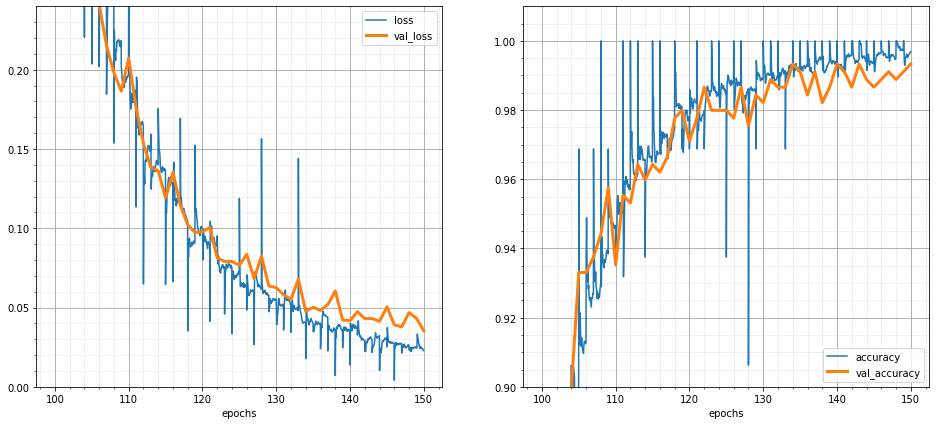
\includegraphics[width=\linewidth]{Immagini/bn}
	\caption{Graph of the third run}
	\end{center}
\end{figure}
\begin{table}[H]
	\centering
	\begin{tabular}{cccccc}
		\textbf{Run} &\textbf{Loss}&\textbf{V.Loss} &\textbf{Acc.}&\textbf{V.Acc.}&\textbf{$\Delta$ Acc.} \\ \hline
	1   & 0.0276    & 0.0439    & 0.9962    & 0.9933    & 0.0029\\
	2   & 0.0255    & 0.0510    & 0.9962    & 0.9888    & 0.0074\\
	3   & 0.0227    & 0.0353    & 0.9969    & 0.9933    & 0.0036\\
	\textbf{Avg} & \textbf{0.0253}    & \textbf{0.0434}    & \textbf{0.9964}    & \textbf{0.9918}    & \textbf{0.0046}\\ 
	\end{tabular}
\end{table}

This iteration of the model adds batch normalization in order to further improve general performance.\\
Adding batch normalization caused the model the train much faster, but this presented a problem: the training was very biased towards the training set from the first epoch. This led to a very big gap in validation and train accuracy, in the order of 0.75 against 0.14 after the first epoch.\\
To counter this negative effect, the starting learning rate was reduced to 0.00005, which allowed for much better results. The slower learning called for an increased number of epochs.




